\documentclass[a4paper]{article}
\usepackage{fullpage}
\usepackage[utf8]{inputenc}
\usepackage[english]{babel}

\usepackage[numbers]{natbib}
\usepackage{amsmath}
\usepackage{float}
\usepackage{graphicx}
\usepackage{listings}
\usepackage{numprint}
\usepackage{tikz} \usetikzlibrary{trees, positioning, arrows.meta}
\usepackage{titlesec}
\usepackage{url}
\usepackage{wrapfig}
\usepackage{xspace}

\lstset{% parameters for all code listings
  language=Python,
  frame=single,
  columns=fullflexible,
  basicstyle=\small
}
\usepackage[autostyle]{csquotes} % fixes quote directions
\MakeOuterQuote{"}

% figure numbers reset each section
\usepackage{chngcntr}
\counterwithin{figure}{section}
\counterwithin{equation}{section}

% Custom macro for including images, \mfigure{img-name}{caption}
\newcommand{\jpgfigure}[2]{
\begin{figure}[H]
    \centering
    \includegraphics[width=\textwidth,height=0.30\textheight,keepaspectratio]{figures/#1.jpg}
    \caption{#2}
    \label{fig:#1}
\end{figure}
}

\newcommand{\pngfigure}[2]{
\begin{figure}[H]
    \centering
    \includegraphics[width=\textwidth,height=0.30\textheight,keepaspectratio]{figures/#1.png}
    \caption{#2}
    \label{fig:#1}
\end{figure}
}

\newcommand{\vgg}{VGG-16\xspace}
\newcommand{\anet}{AlexNet\xspace}
\newcommand{\gnet}{GoogLeNet\xspace}
\newcommand{\inet}{ImageNet\xspace}

\newcommand{\isize}[1]{$#1 \times #1$}

\title{Machine Learning \\ Project Report by Group 6}
\author{Diego Castillo \and Ankur Shukla \and Tristan Wright }
\date{\today}

\begin{document}

\maketitle

\section{Abstract}

% what is the problem?
%How did you solve it?
In 2014 Kaggle organized galaxy zoo challenge to analyze a galaxy image and find the probability that it belongs in a particular class. Classification for training images into 37 different was done by humans in a crowd sourced volunteer effort. Deep convolutional neural network comes to the rescue for this image recognition problem as it learns to recognize components of an image and to combine these components to recognize larger structures in an image. Our choice of architecture for CNN model was VGG-16.
% what are the results?

%conclusion
\section{Introduction}

% Why do we study galaxies?
A galaxy is a system of stars, dust, and matter grouped together by some center of mass. By studying galaxies, astronomers search for answers to questions like "are all galaxies the same size?" and "how and when did galaxies form?" Through the search for these questions scientists learn about the history of the universe and about the origins of our own galaxy.

% Why does it need to be automated?
% Why is machine/deep learning a suitable candidate solution?

As a consequence of this search for questions regarding heavenly bodies, astronomy is a research field ripe with large datasets \cite{microsoft-galaxies}. Simultaneous to the enormous datasets, machine learning methods are rapidly becoming a go-to tool for automating data-intensive processes which normally require days or weeks of --often tedious-- human processing. Due to the incomprehensible size of the Universe, classifying celestial bodies is an excellent candidate for the application of machine learning.

The Sloan Digital Sky Survey (SDSS) has made machine learning methods more viable by releasing large datasets to the public. Since SDSS' inception in 1998 and the first data release in 2000, the group has released over 14 datasets for public use. These datasets have been used for numerous applications of machine learning in the classification of astronomical bodies. For example, \citeauthor{svn-galaxy} in \citeyear{svn-galaxy} used support vector machines to classify galaxies and stars. However, they found in the end that they only preformed marginally better than template matching, a traditional image analysis method \cite{svn-galaxy}. Decision trees have also been employed on the star-galaxy classification problem \cite{ball-decision-trees}. Thanks to more available computing resources in this century, artificial neural networks have been trained to classify galaxies and even detect black holes by analyzing images taken on the X-ray spectrum \cite{black-holes}. Convolutional neural networks (CNN's) have been a popular choice for classifying astronomical images due to their ability to extract features from images which humans might not otherwise select \cite{cnn-star-galaxy}.

This paper demonstrates how a CNN can be constructed to analyze images of galaxies to automatically detect metrics that reproduce the probability distributions derived from expert and crowd-sourced human classifications.

The dataset comes from the Dark Energy Camera Legacy Survey (DECaLS), a subset of an SDSS dataset for specifically galaxies called "Galaxy Zoo". DECaLS uses a larger telescope, so it is 10 times more sensitive to light than the survey that supplied images to the first iteration of Galaxy Zoo. This means there is more detail \cite{zooniverse}. In 2014 this same dataset was used as the premise for a Kaggle competition.

% Finally the economic incentive. By using machine learning for this task we are freeing up the man-hours of dozens if not hundreds of astrophysics PhD students whose sole existence is to categorize galaxies, quasars, and red giants for their thesis advisors. In this manner we follow the footsteps of Bertrand Russel who advocated for shorter working hours in American industrial revolution of the 20th century \cite{russell-idleness}. Today, thanks to the increasing plurality of machine learning tools we are again questioning what is a necessary weekly hourly allocation of work.

\section{The Dataset}

The "Galaxy Zoo" dataset consists of a total \numprint{141553} images. These are split into \numprint{61578} images for training --each with their respective probability distributions for the classifications for each of the inputs-- and \numprint{79975} images for testing.

As a crowd-sourced volunteer effort, images of the dataset were classified across 11 different categories. Each of categories have attributes which volunteers can rank, there are 37 attributes in total. Some categories are dependent on the presence of others, for example number of spiral arms and spiral tightness is dependent on if the galaxy has spiral shape. The votes on these volunteer categorizations are normalized to a floating point number between 0 and 1 inclusive. A number close to 1 indicates many users identified this category for the galaxy image with a high level of confidence, while numbers close to 0 indicate otherwise. These numbers represent the overall morphology of a galaxy in 37 attributes.

Due to these probabilities being tied to each image this is a regression problem rather than a classification problem. Therefore, the task is to determine the degree to which a galaxy has certain attributes and mimic how people would classify the same galaxy.

\section{Theory}

\subsection{Neural Network}

% What is a NN?
% How are they structured?
A standard neural network (NN) consists of many simple, connected processors called neurons. Each neuron produces a sequence of real-valued activations. A neuron can be activated from an input or another neuron's activation through its weighted connections from a previous layer \cite{NeuralNetwork}.

% Visual explanation of a NN
Figure \ref{fig:neural-network} shows how a NN receives a number of inputs which are connected to an activation function through weighted edges. A NN can have any number of inputs, hidden layers, or outputs.

\begin{figure} \label{fig:neural-network}
\centering
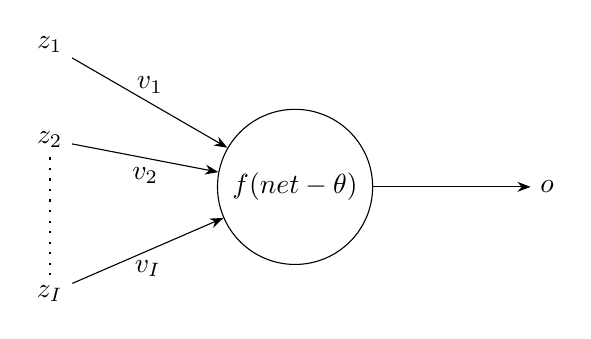
\begin{tikzpicture}[
  mycircle/.style={
     circle,
     draw=black,
     fill=white,
     inner sep=4pt,
     minimum size=20pt},
  mylabel/.style={font=\bf},
  myarrow/.style={-Stealth},
  node distance=1.5cm and 2cm
  ]
  \node[mylabel] (z1) {$z_1$};
  \node[mylabel,below=0.75cm of z1] (z2) {$z_2$};
  \node[mylabel,below=0.25cm of z2] (z3) { };
  \node[mylabel,below=1cm of z3]    (zn) {$z_I$};

  % neuron and output
  \node[mycircle, right=of z3] (neuron) {$f(net - \theta)$};
  \node[mylabel,  right=of neuron] (out) {$o$};

% edges
\draw [myarrow] (z1) -- node[above] {$v_1$} (neuron);
\draw [myarrow] (z2) -- node[below] {$v_2$} (neuron);
\draw [myarrow] (zn) -- node[below] {$v_I$} (neuron);

\draw [myarrow] (neuron) -- node[sloped] {} (out);

\path[] (z2) edge[thick, dash pattern=on \pgflinewidth off 3pt] node[] {} (zn);

\end{tikzpicture}
\caption{A NN which receives the inputs $z_1, z_2, ..., z_I$ and connects them to the neuron through the weighted edges $v_1, v_2, .., v_I$. The input values are multiplied by their respective weights and subtracted from a threshold ($\theta$). The result is passed to an activation function which produces the output \cite{Engelbrecht}.}
\end{figure}

% What is an activation?
% Define ReLU
An activation function computes a weighted sum of its input, adds a bias and decides whether the neuron's value should be propagated or not. A common choice for an activation function is the Rectified Linear Unit (ReLU) \cite{Relu}. A ReLU is defined as: $\sigma(x) = \max(0, x)$, where $x$ is the weighted sum of the inputs. It returns an output $x$ if $\sigma(x)$ is positive, $0$ otherwise. NN's using primarily ReLU activation functions have been shown to enable faster training even with many layers \cite{cnn-star-galaxy}.

\begin{figure}\label{fig:relu}
\centering
\begin{tikzpicture}[y=.4cm, x=0.4cm]
  %axes
  \draw [<->] (-10,0) -- coordinate (x axis mid) (10,0);
  \draw [->]  (0,0) -- coordinate (y axis mid) (0,10);

  %ticks
  \foreach \x in {-8,-6,...,8}
    \draw (\x,1pt) -- (\x,-3pt)
    node[anchor=north] {\x};

  \foreach \y in {2,4,...,8}
    \draw (1pt,\y) -- (-3pt,\y)
      node[anchor=east] {\y};

  % line
  \draw[blue] (-10,0) -- coordinate (x axis mid) (0,0);
  \draw[blue,thick, ->] (0,0) -- coordinate (y axis mid)(10,10);
\end{tikzpicture}
\caption{A ReLU function \cite{reluimage}.}
\end{figure}

It is possible for ReLU to introduce dead neurons whose output is always zero, this problem is known as the dying ReLU problem. To mitigate this issue, a slightly different version of ReLU known as leaky ReLU can be used. Leaky ReLU is defined in equation \ref{leaky-relu}.

\begin{equation}
\sigma(x) =
\begin{cases} \label{leaky-relu}
    x      , & \text{if } x\geq 0\\
    0.01x , & \text{otherwise}
\end{cases}
\end{equation}

Difference between the actual and predicted output (the error) is computed by loss function. In a NN, a loss function is used to correct weights after a feed forward operation, this process of correction is called back propagation. The error is propagated backwards from the output layer through the hidden layers to the input layer, wherein the weights and biases are modified in such a way that the error for the most recent input is minimized. Over many training samples the loss function will minimize error and the value of the weights for the whole network will begin to converge. The curve which the error rate of the network experiences is controlled through a gradient descent method. This method can help determine whether the network should be trained further or to stop early.

% TODO: more about gradient descent and early stopping, mention local minima

\subsection{Deep Learning}
% What is deep learning?
Deep learning is a set of algorithms in machine learning that attempt to learn in multiple levels, corresponding to different levels of abstraction. It is based on learning several levels of representations, corresponding to a hierarchy of features, where higher-level concepts are defined from lower-level ones, and the same lower level concepts can help to define many higher-level concepts. It typically uses artificial neural networks. An observation (e.g., an image) can be represented in many ways (e.g., a vector of pixels), but some representations make it easier to learn tasks of interest through examples (e.g., is this the image of a human face?). Research in this area attempts to define what makes better representations and the best methods for a NN to approach learning them \cite{DeepLearning}.

\subsection{CNNs}

% What is a CNN?
% What was it inspired by?
% When was this architecture created?
A CNN is a type of deep feed-forward neural network~\cite{cnn-star-galaxy} which is able to extract elementary visual features from its input. The creation of CNNs was motivated by Hubel and Wiesel's discovery in~\cite{hubel-wiesel-receptive-fields}, where they were able to find that a cat's visual cortex has locally sensitive, orientation-selective neurons. CNNs were first introduced in \citeyear{Lecun99objectrecognition} \cite{Lecun99objectrecognition}, and since then have been applied to solve numerous different type of problems in natural language processing \cite{Collobert:2008:UAN:1390156.1390177}, image recognition \cite{cnn-star-galaxy}, and recommendation systems \cite{NIPS2013_5004}.

% What is the input of CNN?
% What is a convolution?
% What are CNNs made of?
% What are convolutional layers?
% What are filters?
% What are feature maps?
A CNN takes an image as an input and feeds it through several layers; usually convolutional layers with ReLU activation functions, pooling layers, and a fully-connected layer (FCL). Convolutions are the primary operation of a CNN and what makes them distinct from other type of networks. A convolutional layer parameters is made up of a set of small learnable weights known as filters. A filter has a local receptive field, and given an image as an input to a convolutional layer, it convolves each filter across the image's width and height using a specified stride size and produces outputs called feature maps \cite{cnn-star-galaxy}. Filters are what allow a CNN to learn to extract visual clues from its input such as edges, lines, and corners \cite{Lecun99objectrecognition}. Equation \ref{cnn:feature-map} from \cite{cnn-star-galaxy} gives the mathematical definition of a feature map $k$. The summation is performed over the set of input feature maps, the symbol $*$ describes the convolution operator, and $\boldsymbol{x}_m$ the filters.

\begin{equation} \label{cnn:feature-map}
y^k = \sigma{\bigg(\sum_{m} \boldsymbol{w}^{k}_{m} * \boldsymbol{x}_m + b^k \bigg)}
\end{equation}

% Why ReLU as activation functions?
The filters of a CNN compute linear element-wise multiplication and additions to create the feature maps. In order to add non-linearity, it is common for the convolutional layers to use ReLUs as the activation function which additionally allow for faster training in networks with many layers \cite{cnn-star-galaxy}.

% What is a pooling layer?
% How does a pooling layer work?
% How does a CNN reduce dimensionality?
Feature maps are then fed through pooling layers. A pooling layer is typically of size~$2 \times 2$~\cite{NIPS2012_4824}, and its job is to essentially reduce the resolution of the previous feature map. A pooling layer performs an operation such as selecting the maximum value within its range, thus acting as a regularization technique to avoid overfitting.

% Why a fully-connected layer?
Finally, convolutional and pooling layers are followed up by a FCL. The FCL size needs to be the same as the number of classes or outputs the network has to learn to identify~\cite{Ciresan11flexible}, and its goal is to simply act as a classification layer which outputs the probability for each class.

% How are CNNs trained?
Once the architecture of a CNN has been specified, its filters and weights are initialized to small random values. Next, given an image as an input, it is fed through the convolutional, pooling operations, and the FCL. The output probabilities of the network are then used to compute the total error, and finally gradient descent is used to update the filter and weight values with respect to their contribution to the total error. This process is repeated with other images in the dataset until satisfactory results are achieved.

\section{Implementation}

Data pre-processing, CNN setup, training, test, overfitting, data augmentation...

\section{Results}

%"We don't care much about results, except when they're bad." - Ölle

% save me I'm useful somewhere
% \begin{equation}\label{rmse}
% RMSE(y,\hat{y}) = \sqrt{\frac{1}{n}  \sum_{i=1}^{n} (y_i - \hat{y}_i)}
% \end{equation}

Each model was trained for at most fifty epochs on the full training dataset. Early runs were trained with a 90/10 training-validation split, there didn't seem to be much room for improvement based on the separation between the validation and training loss. Thus, an 80/20 split was settled on, results were much better. Early stopping would be invoked if validation loss did not improve for five epochs. To make sure the results could be equally quantified the dataset was shuffled with the same random seed each time.

\subsection{Benchmarks}\label{benchmarks}
The Galaxy Zoo Kaggle competition has a test image set of \numprint{79975} images. After training the model the network uses these images to produce predictions. These predictions are saved as a CSV file and uploaded to Kaggle. Kaggle then scores the predictions using the root mean square error (RMSE) between the model predictions and what the actual values are (these actual values for the test set are kept secret), the lower scores are better. There are certain basic thresholds which can be used to determine if the model behaves as a random classifier or worse. The first is an All Zeros benchmark, this is equivalent to a network that always outputs zeros for all attributes. Similarly, there is an All Ones benchmark; these two benchmarks represent random classifications which, while not entirely trivial to pass, require some rational architectural choices. The final benchmark is harder, a Central Pixel benchmark, which are the predictions if the outputs were simply the central pixel RGB value in each training image. Very early implementations of the VGG16 model could pass the All Zero benchmark, later--with the right hyper-parameters-- the model could pass the All Ones and Central Pixel benchmarks. Results through the rest of this paper are based on the RMSE score Kaggle given for a particular model.

\subsection{Performance}

Before immediately attempting data-augmentation methods, a few hyperparameter configurations were run to get a better idea of the best input size and the best batch size for moving forward (figure \ref{tab:plain_results}).

\begin{table}[]
    \centering
    \begin{tabular}{|r|c|c|}
        \hline
                      & \isize{69} & \isize{106} \\ \hline
        Batches of 16 & 0.11538 & 0.11062 \\ \hline
        Batches of 32 & 0.11476 & 0.11288 \\ \hline
    \end{tabular}
    \caption{Spread of results for various input and batch sizes. In the Kaggle competition this would score 78, 88, 94, 95th place respectively.}
    \label{tab:plain_results}
\end{table}

Results where image size was \isize{69} and where the batch size was 32 or 16 the loss graph and validation loss exhibited traits of overfitting (figure \ref{fig:32b-69}). The results from Kaggle may, in fact, back this up, as the score gets better the larger the batch size. Although, two points don't necessarily make a trend, it could also be that larger batch sizes may be necessary when the images (input sizes) are smaller.

\pngfigure{32b-69}{The training loss line being lower than the validation loss line is characteristic of overfitting. Stopped before 50 epochs.}

\pngfigure{32b-106-90-10}{A run with a 90/10 training-validation split, the score from this run was admissible but ultimately beat by 80/20 splits. The Kaggle score from this run was $0.13070$.}

% This figure feels a little redundant
\pngfigure{32b-106-80-20}{A run with 80/20 training-validation split. Notice the smoother curve versus a run with the same parameters but a 90/10 split.}

Results for the larger images are more in line with expectations. Interestingly, the smaller batches of 16 worked better than 32. This may be surprising compared to the original VGG-16 implementation where input sizes were \isize{224} and their batch was 256. The low learning rate is potentially the parameter solving this. Again, the ImageNet dataset is a little more than an order of magnitude larger than the Galaxy Zoo one, in this aspect the chosen architecture may be overkill and a smaller VGG variant should have been tried out first.

The best run was a simple improvement from an early run where the data was split 90/10 (figure \ref{fig:32b-106-90-10}). This was a rather high split, while it could be trained further the jitter of the validation loss line is cause for concern. It was eventually settled on using the same split which VGG did: 80/20. The results of this run produce an error curve smoother than the one a 90/20 split produced and one which, if desired, could continue to be trained (figure \ref{fig:32b-106-80-20}).

\subsection{HSV Input format}

In digital imagery pixels are stored as combinations of three values red, green, and blue (RGB). However, there are many more ways to represent color; in printing for example: cyan, magenta, yellow, black (CMYK) are optimal values because of how light reflects on printed surfaces. Hue, saturation, value (HSV) is a different color space where the color is stored in hue, color intensity is stored in saturation, and the brightness is stored in a value. There were hypothesis if converting the galaxy images to this color format might enhance responses in the network, stars being bright, the star pixels will emit a high $V$ value and thus create stronger weights.

The results from this color space conversion were not terrific. With a batch of 32 with images the image size of \isize{106} got a score of $0.13778$ worse than any RGB result. The score was worse due to two issues over which there was much rumination. While $V$ may have been regularly high for the features the model is trying to detect, $H$ may have been too varied for the network to converge on. For $S$, the color intensity of images was not very high, and so most colors were close to zero on the saturation scale. The combination of a rapidly fluctuating variable $H$, a regularly small value of $S$ made $V$ comparatively worthless to the network. This score would have earned 178th in the Kaggle competition.

\subsection{Data Augmentation}
After the examining the results on 32 and 16 batches it was decided to move forward with applying data augmentation to image sizes of \isize{106}. Augmenting with the transformations discussed in section \ref{aug} effectively increases the training data set by a great amount. In an 80/20 split there will be \numprint{49262} training images, when this is augmented there will effectively be \numprint{788198} images. The validation dataset is not augmented as it is needed as unaltered images are best used for a baseline.

\begin{table}[]
    \centering
    \begin{tabular}{|r|c|}
        \hline
                      & \isize{106} \\ \hline
        Batches of 16 &  0.11331 \\ \hline % 91
        Batches of 32 &  0.11673 \\ \hline % 97
    \end{tabular}
    \caption{Spread of results for various batch sizes with data augmentation. Augmentation was a random combination of reflection on the horizontal or vertical axis and being rotated by 90 degree increments. }
    \label{tab:aug_results}
\end{table}

This reinforces a forming hypothesis that smaller batch sizes for the \isize{106} image sizes are more optimal. These scores would have earned 91st and 97th respectively. There may be too much augmentation going on and not enough hyperparameter adjustment. There are almost a three quarters of a million images with these transformations, it might have been best to perform some learning rate studies; as is, the network might not have taken the large strides it needed to attain better score than the un-augmented datasets.

\begin{table}[]
    \centering
    \begin{tabular}{|l|c|}
        \hline
        \multicolumn{2}{|c|}{\textbf{All results, sorted best to worst}} \\ \hline
        \textbf{\textit{image size}}, \textbf{\textit{batch size}} & \textbf{Score} \\ \hline

        \isize{106}, 16 & 0.11062 \\ \hline
        \isize{106}, 32 & 0.11288 \\ \hline
        \isize{106}, 16, augmented   & 0.11331 \\ \hline
        \isize{69}, 32 & 0.11476 \\ \hline
        \isize{69}, 16 & 0.11538 \\ \hline
        \isize{106}, 32, augmented   & 0.11673 \\ \hline
        \isize{106}, 32, 90/10 split & 0.13070 \\ \hline
        \isize{106}, 32, HSV format  & 0.13778 \\ \hline

    \end{tabular}
    \caption{All results sorted by Kaggle score. Runs are using 80/20 split unless specified otherwise.}
    \label{tab:all_results}
\end{table}

\section{Discussion}

From the get-go, there were a lot of models and solutions for this problem available online to trawl over and gain knowledge from. In that sense we stood on the shoulders of giants, and tall giants they were. To summarize, we implemented a sixteen layer CNN and trained it on a dataset of tens of thousands of images. These images were cropped and down-sampled to reduce dimensionality and make them a manageable size for the network. From those initial scores a series of other methods were tried and explored from data-augmentation to color space shifting. In the end the initial trials were the most successful. 

\subsection{Further Work}
A top 100 score on Kaggle is an accomplishment but there is plenty of improvement to be done. Hyperparameter studies beyond batch sizes and training splits were not performed, it is probably that parameters like learning rate and learning rate decay could have helped improve the network past current thresholds. Essentially, the problem was many runs with varying methods producing varying results; instead of trying to laser in on a single great score by perpetually improving a single good result. We took a few props from the winning Kaggle submission, what else could we garner from their solution? A smaller network for one, feeding images of \isize{69} through such a large network might have been the folly of those runs which ultimately led to overfitting, there were simply too many network parameters and not enough input parameters to fill them. Follies with data-augmentation may not have been negligible either, while our images were certainly rotationally invariant , we may have performed too many translations and made the apparent dataset too large for the network to settle on. Tweaking the learning rate and number of epochs could have worked well, though in that scenario with resources limited as they were, there might not have been time to sufficiently explore that line of experimentation which would have involved running 8-12 hour jobs.

With the network as it is, could there be other astronomical problems to tackle? In the coming years the James Webb space telescope will soon be launched (or hopefully, it's already been delayed multiple times this decade). An infrared telescope, it will be able to see objects in the universe which conventional visible light telescopes cannot. This could open up whole new bodies previously obscured by dust and nebulae. Notable here, it will be able to detect the earliest galaxies in our universe. We could also probably classify cats.

\subsection{Contributions}
Diego kept us organized and wrote initial code for training and validation splitting. Ankur wrote and gathered the many valuable research materials.
Tristan coded and babysat the multi-hour runs. Everyone wrote lots in this paper.

\bibliographystyle{plainnat}
\bibliography{references}
\end{document}
